\documentclass[a4paper,10pt,oneside]{article}
\usepackage[polutonikogreek,italian]{babel}
\usepackage[utf8x]{inputenc}
\usepackage{amsmath}
\usepackage{amsthm}
\usepackage{amssymb}
\usepackage{amscd}
\usepackage{graphicx}
\usepackage{float}
\usepackage{array}
\usepackage{rotating}
\usepackage[small]{caption}
\usepackage{lscape}
\usepackage{fancybox}
\usepackage{booktabs}
\usepackage[noanswer]{exercise}
\usepackage{wasysym}

\def\Arrow{\raisebox{-.5\height}{\scalebox{4}{$\Rightarrow$}}}
\parindent0ex
\renewcommand{\fboxsep}{0.4cm}
\usepackage{hyperref}
\renewcommand{\textfraction}{0.05}
\renewcommand{\topfraction}{0.95}
\renewcommand{\bottomfraction}{0.95}
\renewcommand{\floatpagefraction}{0.35}
\renewcommand{\ExerciseName}{Esercizio}
\renewcommand{\ExerciseListName}{Es}
\setcounter{totalnumber}{5}
\restylefloat{figure}
\begin{document}
\thispagestyle{empty}

\begin{center}
{\huge \textbf{Laboratorio analisi dati}}
\end{center}

\vspace{1cm}

\begin{abstract}
Calcolo numerico di velocità ed accelerazione, esempio di utilizzo del programma Open Source \emph{Tracker} per l'analisi fisica del moto di un proiettile da un filmato ripreso in laboratorio.

\end{abstract}

\section*{Calcolo numerico di velocità ed accelerazione}
In laboratorio effettueremo misure di posizione sia attraverso dei filmat che con i sensori di moto ultrasonici della Pasco, i dati raccolti saranno delle lunghe serie di coppie ordinate del tipo $(t_i,x_i)$, i sensori a nostra disposizione effettuano misure ad intervalli di tempo costanti (da $5\ Hz$ a $120\ Hz$ per i sensori Pasco e fino a $1000\ Hz$ per la macchina fotografica) i  dati raccolti saranno generalmente esprimibili come $(\Delta t\cdot i,x_i)$ dove l'indice $i$ indica l'i-esima misura.
Dalla teoria studiata in classe sappiamo che:
\begin{equation}
 v_x(t)=\lim _{\Delta t \to 0} \frac {\Delta x}{\Delta t}
\end{equation}
chiaramente questa formula non è applicabile ad un sistema reale dato che non è materialmente possibile effettuare misurazioni della posizione ad intervalli di tempo arbitrariamente piccoli. La velocità che andremo a calcolare sarà quindi rappresentata nel nostro grafico $(t,s)$ dalla pendenza della spezzata che congiunge due punti (misure). Il valore che otterremo dal calcolo sarà quindi una velocità media

\begin{equation}\label{forward_diff}
\overline{v}_x(t_i)=\frac{\Delta x}{\Delta t}=\frac{x_{i+1}-x_i}{\Delta t}
\end{equation}

una stima più accurata della velocità media di un sistema al tempo $t_i$ si può ottenere con una versione simmetrizzata della [\ref{forward_diff}]:
\begin{equation}
 \overline{v}_x(t_i)=\frac{x_{i-1}-x_{i+1}}{2\Delta t}
\end{equation}

notiamo che a differenza di quanto visto a lezione in cui era nota la dipendenza funzionale dello spazio dal tempo (la legge oraria) in questo caso conosciamo unicamente delle coppie tempo-posizione del corpo e tali valori sono affetti da un errore sperimentale non eliminabile figura [\ref{fig:velocita_numerica}]. Alla luce di quanto detto appare chiaro come non sarà mai possibile avere una perfetta corrispondenza tra l'andamento teorico e i dati sperimentali, tutto ciò che saremo in grado di fare sarà stimare la probabilità con cui il nostro modello teorico descrive le osservazioni. Per eseguire una sperimentazione corretta dovremmo tener conto sia dell'errore di misura dei dati iniziali (tempo e posizione) sia dell'errore sulle grandezze derivate (velocità ed accelerazione) amplificato dalle approssimazioni numeriche\footnote{L'errore sulle grandezze derivate sarà inoltre aggravato anche dal sistema fisico (computer) su cui effettueremo i calcoli, sapreste dire perché?}


\begin{figure}[H]
 \centering
 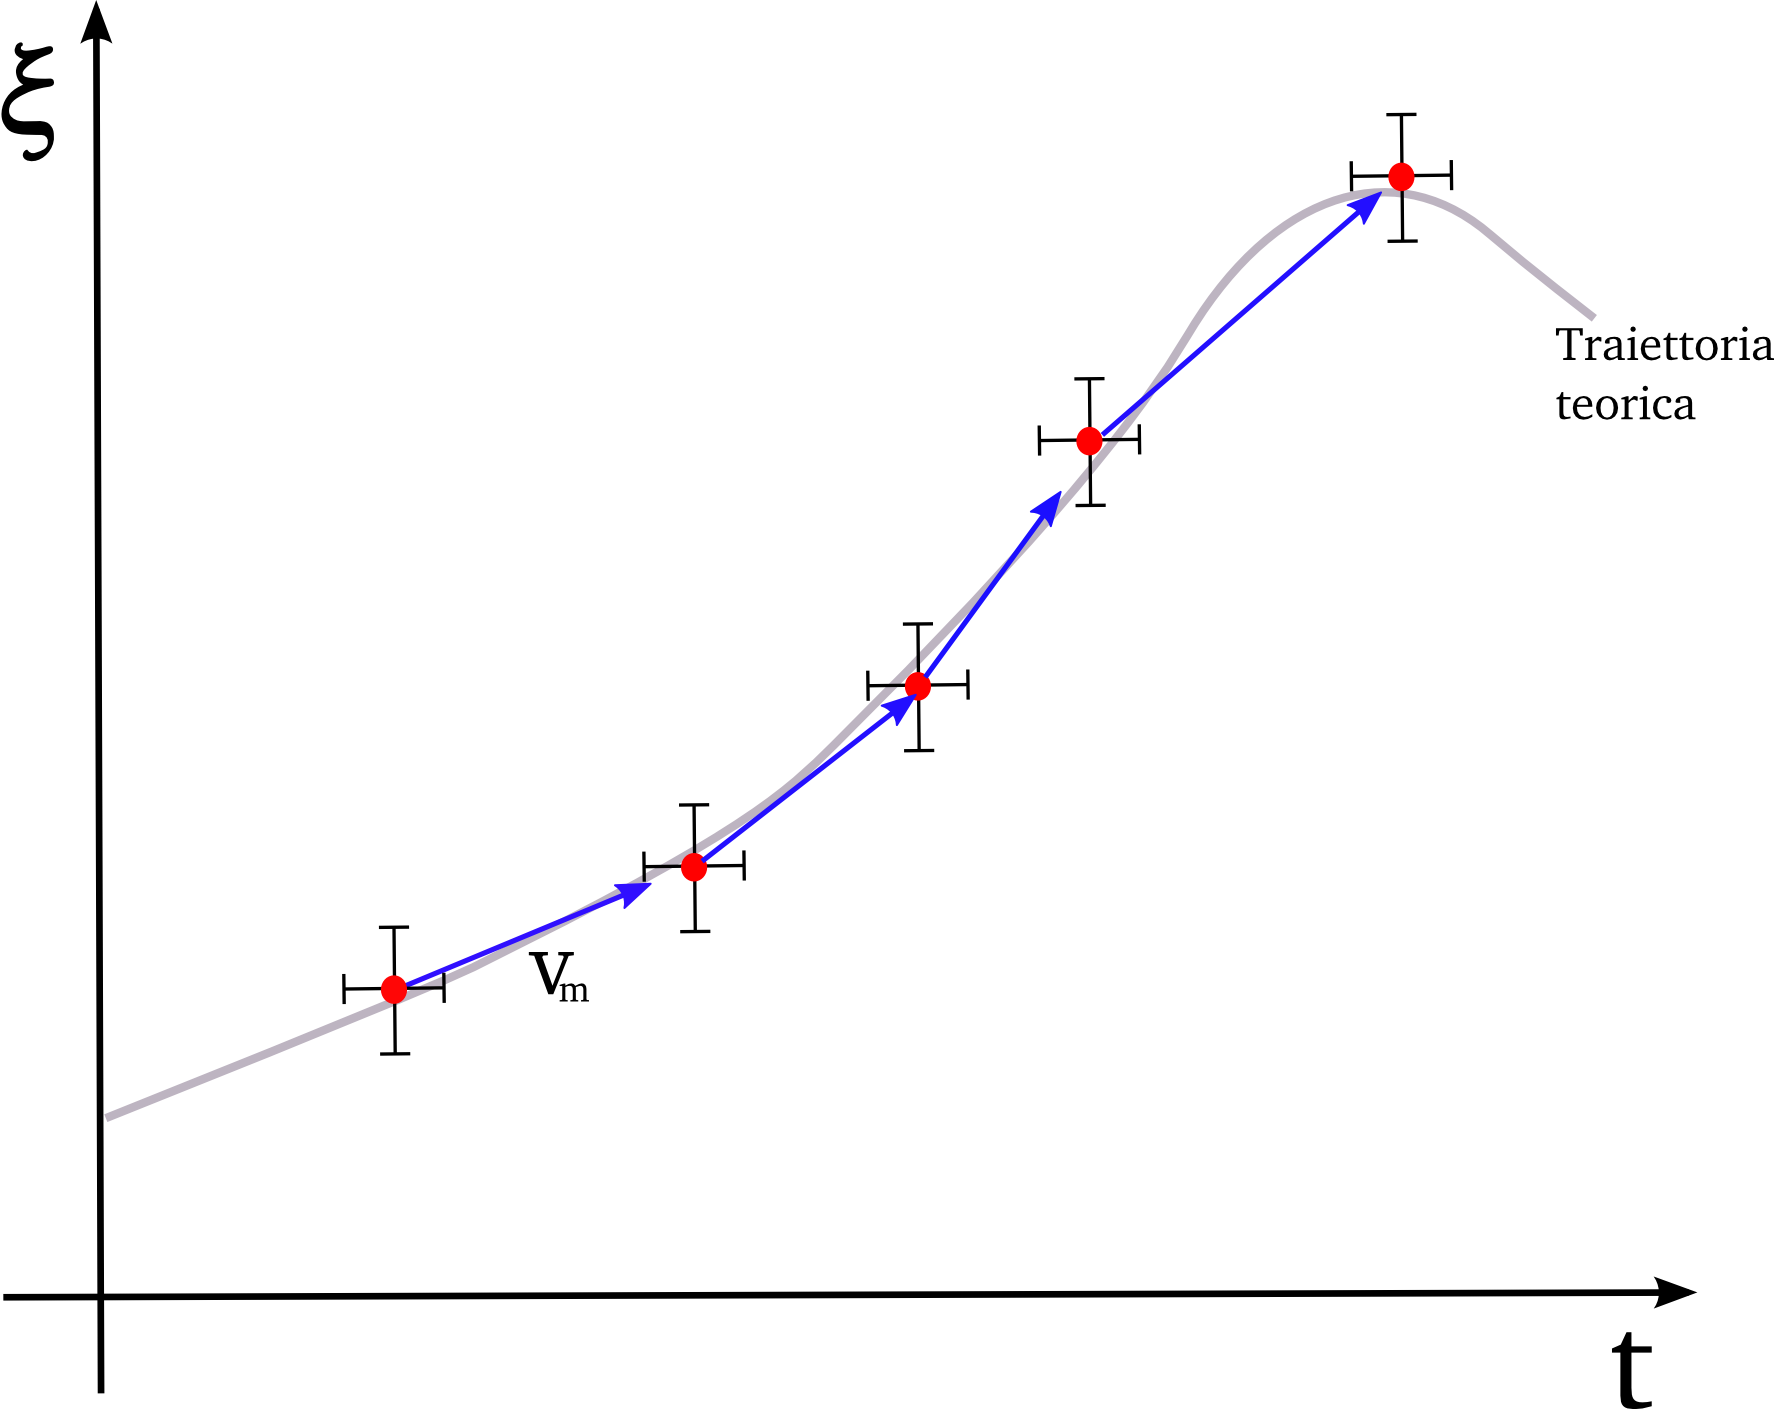
\includegraphics[width=0.8\textwidth]{./immagini/velcita_numerica.png}
 % velcita_numerica.png: 1774x1409 pixel, 300dpi, 15.02x11.93 cm, bb=0 0 426 338
 \caption{La velocità media non è calcolata come coefficiente angolare della secante della curva teorica ma come coefficiente angolare della rette che contiene il segmento che congiunge due misure successive di posizione. Nel grafico $\xi$ è una coordinata spaziale generica}
 \label{fig:velocita_numerica}
\end{figure}


Una volta ottenuta la velocità media possiamo calcolare l'accelerazione media utilizzando una formula analoga alla [\ref{forward_diff}]:
\begin{equation}
 \overline{a}_x(t_i)=\frac{\Delta v}{\Delta t}=\frac{v_{i+1}-v_i}{\Delta t}
\end{equation}
Al termine dei calcoli riporteremo i risultati ottenuti in una tabella e quindi in un grafico che ci aiuterà a visualizzare la dipendenza temporale di accelerazione  e velocità:
\begin{table}[H]
\begin{center}
\begin{tabular}{llll}\toprule
$t_i$ & $x_i$& $\overline{v}_i$& $\overline{a}_i$ \\ \midrule
$0.1s$&$0.3m$&$1ms^{-1}$&$10ms^{-2}$\\
$0.2s$&$0.4m$&$2ms^{-1}$&\ldots\\
$0.3s$&$0.6m$&\dots&\ldots\\
\ldots &\ldots&\dots&\dots \\ \bottomrule
\end{tabular}\caption{Tabella con velocità ed accelerazioni calcolate dalle misurazioni effettuate in laboratorio, notate come con $n$ misure sia possibile calcolare $n-1$ velocità ed $n-2$  accelerazioni utilizzando il metodo delle differenze in avanti}\label{tab:extab1}
\end{center}
\end{table}



\section*{Utilizzo di Tracker}

\subsection*{Traccia \emph{Punto di massa}}


Il programma Tracker che potete scaricare all'indirizzo \url{http://www.cabrillo.edu/~dbrown/tracker/} rappresenterà uno strumento molto utile per l'analisi dei dati che raccoglieremo durante le esperienze di laboratorio \footnote{Per analizzare manualmente il filmato del proiettile potete seguire le note del laboratorio di cinematica dello scorso anno [\cite{Laboratorio7}]}. Vediamo come analizzare una ripresa video del moto parabolico di una pallina lanciata da un cannone ad elastico.
Come prima cosa dobbiamo suddividere in fotogrammi il filmato, a tal fine utilizzeremo ffmpeg che può essere scaricato a questo indirizzo \url{http://www.arachneweb.co.uk/software/windows/avchdview/ffmpeg.html}\footnote{Ffmpeg è disponibile anche in ambiente Mac e Linux, se usate tali sistemi operativi e non riuscite ad installare il programma inviate una richiesta di aiuto tramite il sito \url{http://cartan.e-moka.net}}, se usate un sistema operativo Windows aprite il prompt dei comandi ed entrate nella directory che contiene il file che vogliamo esaminare, quindi digitate il comando
\begin{verbatim}
ffmpeg -i <nome file> fotogramma%03d.png
\end{verbatim}
dove \verb#<nome file># deve essere sostituito con il nome del file in analisi.
Quando ffmpeg avrà terminato la suddivisione del filmato andremo ad aprire Tracker\footnote{Per eseguire Tracker è necessario installare la Virtual Machine Java} e tramite il menu File \RIGHTarrow Apri \footnote{Se l'interfaccia dovesse essere in Inglese potete trasformarla in italiano dal menu Edit \RIGHTarrow language} selezioneremo il file \verb#fotogramma001.png# precedentemente creato da ffmpeg. Tracker caricherà automaticamente tutti i fotogrammi della sequenza in memoria\footnote{se il vostro filmato è lungo Tracker potrebbe occupare molta memoria ram $>1\ Gb$} la schermata del programma dovrebbe apparire come in figura [\ref{fig:tracker_caricamento_immagini_1}].

\begin{figure}[H]
 \centering
 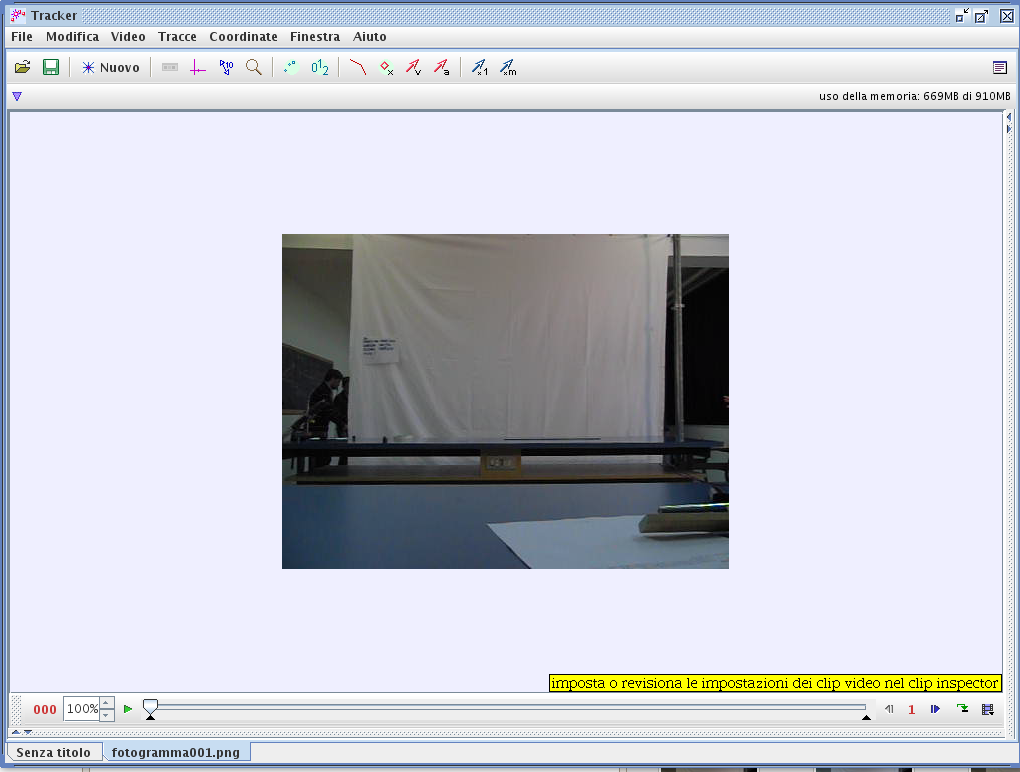
\includegraphics[width=\textwidth]{./immagini/tracker_caricamento_immagini1.png}
 % tracker_caricamento_immagini1.png: 1020x772 pixel, 72dpi, 35.98x27.23 cm, bb=
 \caption{Carichiamo le immagini prodotte con ffmpeg tramite il menu File \RIGHTarrow Apri}
 \label{fig:tracker_caricamento_immagini_1}
\end{figure}

Nella pagine che seguono faremo spesso riferimento alle icone presenti nella barra dei comandi  che potete vedere elencate in tabella [\ref{table:icons}]
\begin{table}[H]
\begin{center}
\begin{tabular}{cp{8cm}}\toprule
\raisebox{-0.5cm}{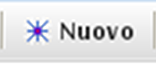
\includegraphics[height=1cm]{./immagini/barra_icone_nuovo.png}}& {\small Pulsante nuovo per la creazione delle traccie}\\[0.5cm]
\raisebox{-0.5cm}{
\includegraphics[height=1cm]{./immagini/barra_icone_sistema_riferimento.png}}& {\small Cliccando su questo pulsante è possibile costruire un sistema di riferimento cartesiano da sovrapporre al filmato}\\[0.5cm]
\raisebox{-0.5cm}{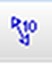
\includegraphics[height=1cm]{./immagini/barra_icone_metro_nastro.png}}&{\small Lo strumento metro a nastro verrà utilizzato per impostare la corretta scala di lunghezze}\\[0.5cm]
\raisebox{-0.5cm}{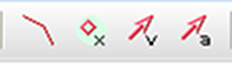
\includegraphics[height=1cm]{./immagini/barra_icone_vettori.png}}&{\small Tramite questi comandi potremmo visualizzare i vettori posizione velocità ed accelerazione sul filmato.}\\[0.5cm]
\raisebox{-0.5cm}{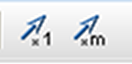
\includegraphics[height=1cm]{./immagini/barra_icone_ingrandimento.png}}& Con questi strumenti potremo modificare la scala di visualizzazione dei vettori e/o moltiplicarli per la massa\\[0.5cm]
 \bottomrule
\end{tabular}\caption{Alcune delle icone nella barra degli strumenti di Tracker}\label{table:icons}
\end{center}
\end{table}


Spesso i filmati fatti in laboratorio potrebbero risultare eccessivamente sottoesposti, Tracker ci da la possibilità tramite il menu Video \RIGHTarrow filtri \RIGHTarrow nuovo \RIGHTarrow brightness
di migliorare la leggibilità delle immagini, immagine [\ref{fig:filtro_luminosita}],  notate che oltre a \emph{brightness} il programma fornisce altri filtri di cui potete trovare una descrizione nel manuale  online.

\begin{figure}[H]
 \centering
 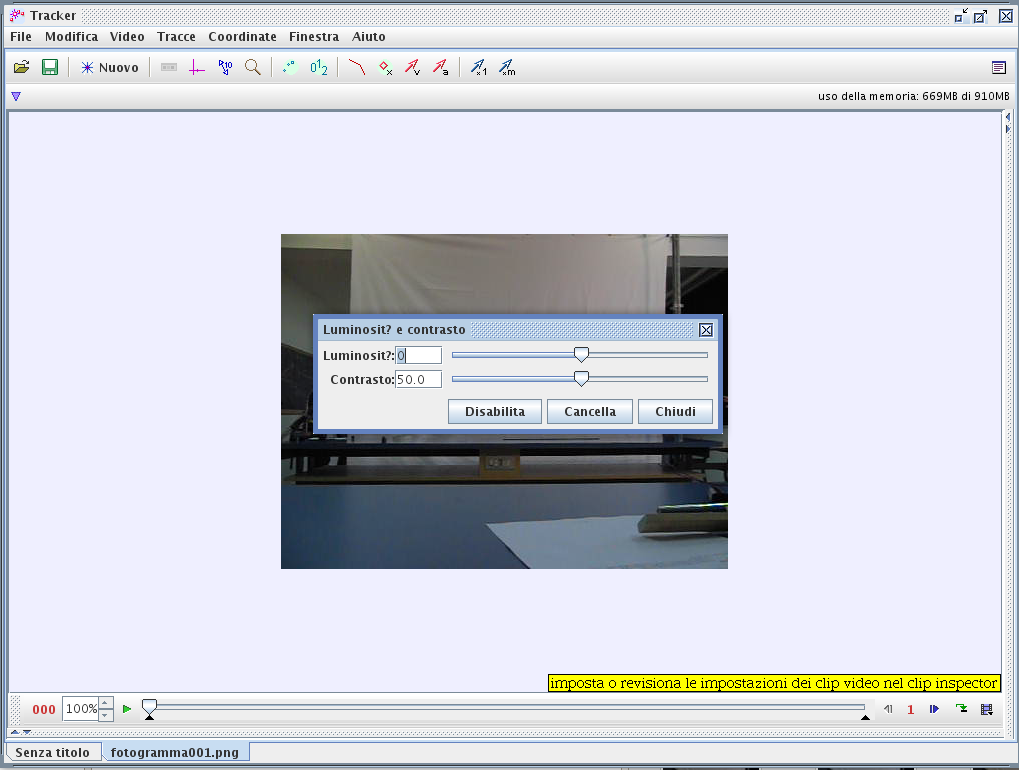
\includegraphics[width=\textwidth]{./immagini/tracker_filtri_luminosita.png}
 % tracker_filtri_luminosita.png: 1019x770 pixel, 72dpi, 35.94x27.16 cm, bb=0 0 1019 770
 \caption{Per evidenziare la posizione del proiettile aumentiamo la luminosità ed il contrasto dell'immagine  Video \RIGHTarrow Filtri  \RIGHTarrow  Nuovo \RIGHTarrow brightness}
 \label{fig:filtro_luminosita}
\end{figure}
Dopo aver aumentato, se necessario, la luminosità dell'immagine impostiamo i parametri del video in Tracker, per poter effettuare delle misure è infatti necessario dichiarare la frequenza e l'estensione temporale della successione di immagini. Cliccando sull'icona presente nell'angolo in basso a destra comparirà una finestra di dialogo dalla quale potremo specificare i parametri video figura [\ref{fig:parametri_video}]



Nel caso in esame abbiamo impostato il campo \textsl{Quadro iniziale} a 355 dato che questo è risultato essere il primo fotogramma utile, il campo \textsl{Quadro finale} a 490 siccome il fenomeno di interesse finiva proprio in tale frame, il campo \textsc{Frequenza di quadro} è stato impostato a 240 dato che la frequenza del filmato era di $240\ Hz$ \footnote{Se il vostro computer è dotate di poca memoria Ram potete cancellare fisicamente dal disco tutte le immagini che non contengono dati interessanti e fornire a Tracker come prima immagine il primo fotogramma di interesse}. Notate inoltre che la dimensione del passo è stata impostata a 5 per limitare il numero di frame da analizzare durante
l'esempio.

\begin{figure}[H]
 \centering
 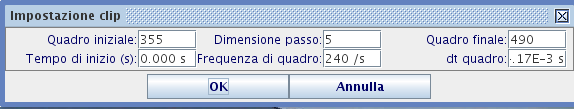
\includegraphics[width=0.8\textwidth]{./immagini/tracker_parametri_video.png}
 % tracker_parametri_video.png: 574x109 pixel, 72dpi, 20.25x3.84 cm, bb=0 0 574 109
 \caption{Impostiamo i parametri video dal menu accessibile tramite l'icona nell'angolo in basso a destra}
 \label{fig:parametri_video}
\end{figure}

Dopo aver impostato i parametri temporali dobbiamo impostare il fattore di scala tra l'immagine e il sistema che questa rappresenta. Tracker ci mette a disposizione lo strumento \textsl{Misura a nastro}, selezioniamolo dalla barra dei menu, sull'immagine comparirà una doppia freccia azzurra che dovremo far coincidere con una struttura di lunghezza nota, nel caso in esame una stecca da $60\ cm$ posta sopra il bancone, una volta terminata questa operazione clicchiamo sulla casella di testo posta sopra il righello e inseriamo la lunghezza nota in metri figura [\ref{fig:righello_dimensione}]. Tracker utilizza delle unità arbitrarie sarà quindi nostra cura far si che tutti i valori specificati siano omogenei.

\begin{figure}[H]
 \centering
 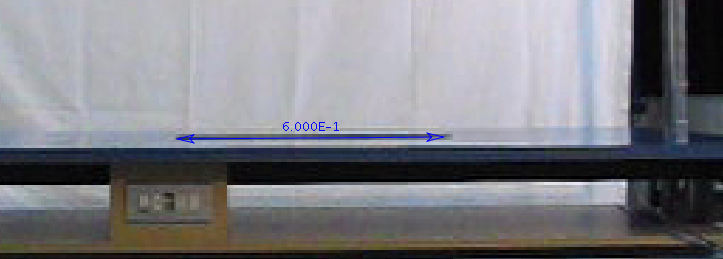
\includegraphics[width=0.8\textwidth]{./immagini/tracker_righello_dimensione.png}
 % tracker_righello_dimensione.png: 723x259 pixel, 72dpi, 25.50x9.14 cm, bb=
 \caption{Per creare una nuova \emph{Misura a nastro - Ruler} clicchiamo sul tasto corrispondente del menu e trasciniamo il righello fino a coincidere con l'oggetto di dimensione nota posto nel campo del filmato}
 \label{fig:righello_dimensione}
\end{figure}

Dopo aver posizionato  la \textsl{Misura a nastro}, per poter ottenere le coordinate cartesiane del proiettile sparato dal cannone, sarà necessario stabilire un sistema di riferimento all'interno dell'immagine. Clicchiamo sullo strumento Assi, tabella [\ref{table:icons}] nella barra delle icone e posizioniamo il sistema di riferimento che comparirà sull'immagine nella posizione che preferiamo figura [\ref{fig:assi_coordinati}]. Nota se il filmato non è perfettamente orizzontale è possibile ruotare gli assi cartesiani agendo con il mouse sulla \emph{maniglia} presente sull'asse delle ascisse.

\begin{figure}[H]
 \centering
 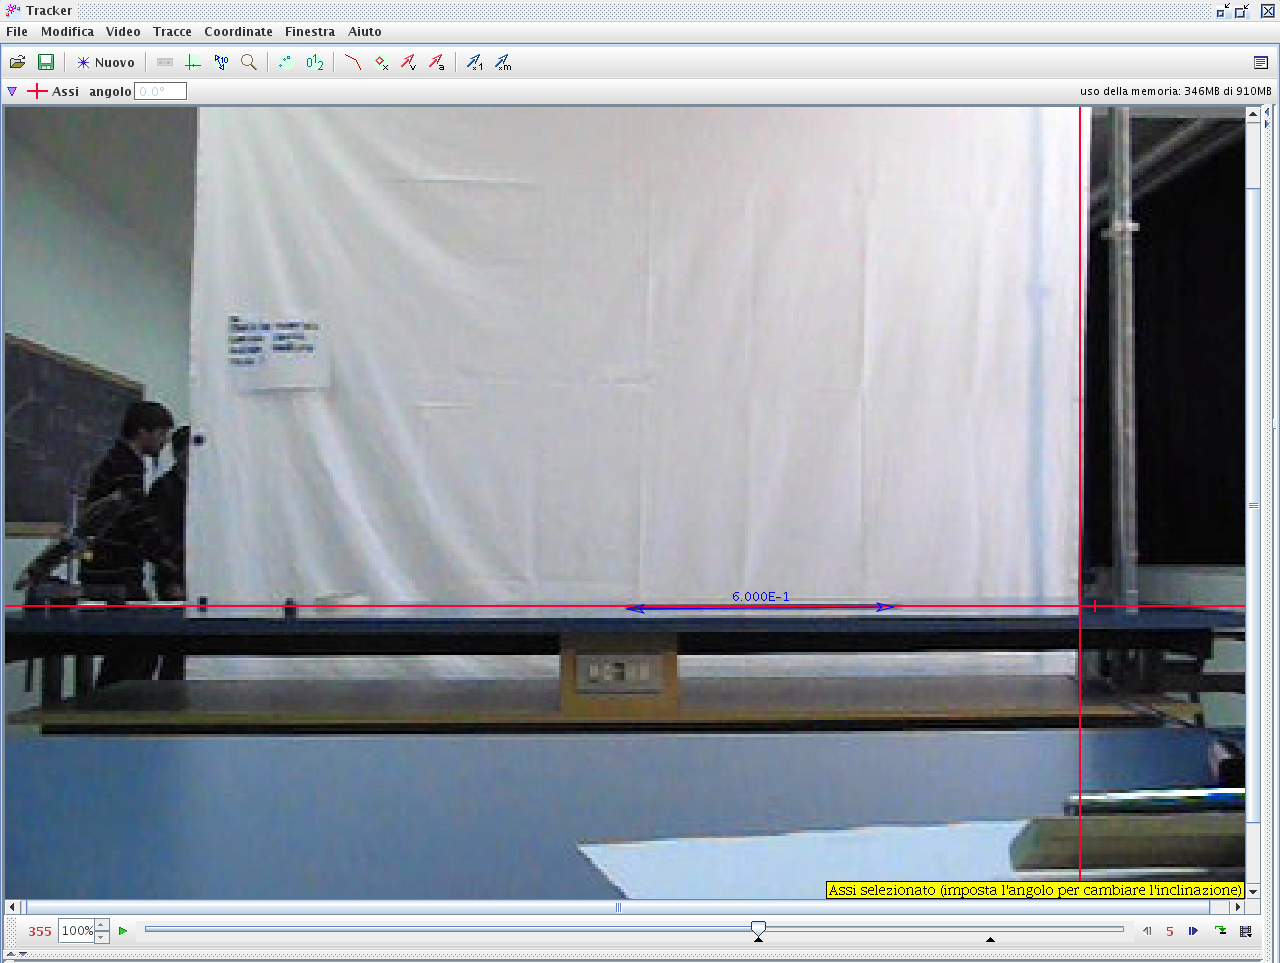
\includegraphics[width=\textwidth]{./immagini/tracker_assi_posizionati.png}
 % tracker_assi_posizionati.png: 1280x963 pixel, 72dpi, 45.15x33.97 cm, bb=0 0 1280 963
 \caption{Posizioniamo gli assi coordinati con il tool apposito nella barra delle icone superiore}
 \label{fig:assi_coordinati}
\end{figure}

Tracker è ora pronto per iniziare l'analisi dei dati. Il nostro scopo sarà identificare in ogni fotogramma la posizione del proiettile ed estrarre, quindi tali coordinate, che verranno poi utilizzate  per il calcolo di grandezze derivate. Ogni successione di posizioni di un oggetto verrà rappresentata in Tracker come una  traccia, nel nostro caso particolare la traccia sarà di tipo \emph{Punto di massa}. Iniziamo creando una nuova traccia cliccando sull'icona \emph{Nuovo} e scegliendo la voce \emph{Punto di massa}, comparirà una nuova finestra con all'interno la traccia appena creata figura [\ref{fig:nuovo_punto_massa}]

\begin{figure}[H]
 \centering
 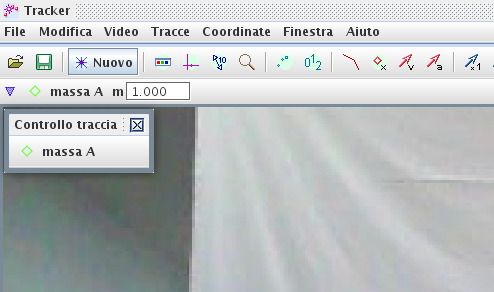
\includegraphics[width=0.8\textwidth]{./immagini/tracker_nuovo_punto_massa.png}
 % tracker_nuovo_punto_massa.png: 494x292 pixel, 72dpi, 17.43x10.30 cm, bb=0 0 494 292
 \caption{Scegliamo Nuovo \RIGHTarrow punto massa dalla barra delle icone}
 \label{fig:nuovo_punto_massa}
\end{figure}

Cliccando sul nome della traccia potrete impostare le caratteristiche grafiche dell'indicatore della traccia, nel nostro esempio si è scelto il cerchio. Per iniziare il riconoscimento, tenendo premuto il tasto \textsl{shift} sulla tastiera, clicchiamo con il mouse sulla prima posizione del proiettile, Tracker avanzerà automaticamente  al fotogramma successivo nel quale ripeteremo l'operazione di riconoscimento, continueremo in questo modo fino all'ultimo fotogramma di interesse (490). Il risultato finale dovrebbe essere simile a quello di figura [\ref{fig:posizioni_massi}]

\begin{figure}[H]
 \centering
 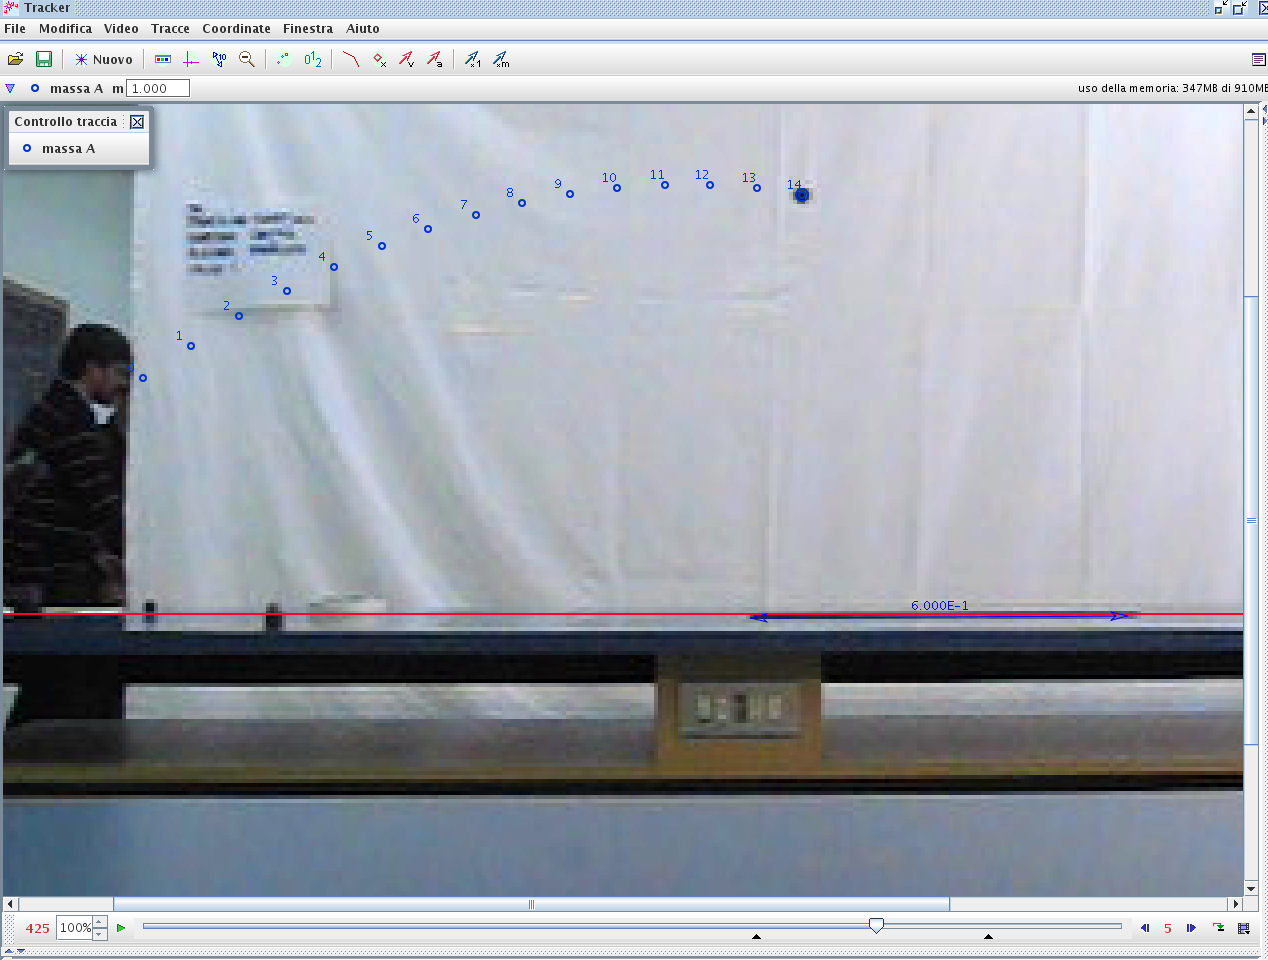
\includegraphics[width=\textwidth]{./immagini/tracker_posizioni_massa.png}
 % tracker_posizioni_massa.png: 1268x960 pixel, 72dpi, 44.73x33.86 cm, bb=0 0 1268 960
 \caption{Tenendo premuto il tasto \textbf{shift} individuate le posizioni dell'oggetto in moto nei vari fotogrammi}
 \label{fig:posizioni_massi}
\end{figure}

La prima parte del lavoro è conclusa, possiamo usare i dati raccolti per visualizzare la traiettoria del proiettile figura [\ref{fig:visualizzazione_traiettoria}], i vettori velocità media figura [\ref{fig:visualizzazione_vel}] e infine i vettori accelerazione media figura [\ref{fig:vettori_acc}]


\begin{figure}[H]
 \centering
 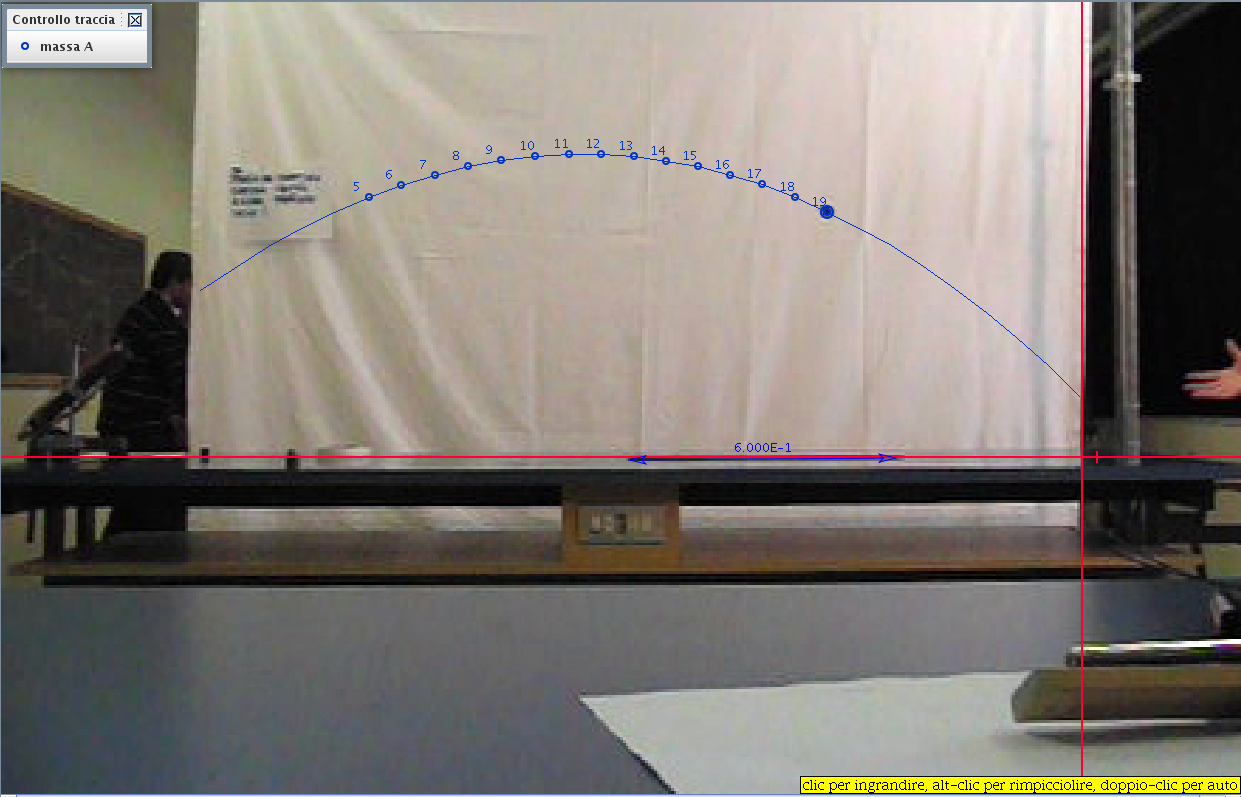
\includegraphics[width=0.8\textwidth]{./immagini/tracker_visualizzazione_traiettoria.png}
 % tracker_visualizzazione_traiettoria.png: 1241x797 pixel, 72dpi, 43.77x28.11 cm, bb=0 0 1241 797
 \caption{Dopo aver effettuato il riconoscimento delle posizioni dell'oggetto nei vari fotogrammi è possibile rappresentare la sua traiettoria}
 \label{fig:visualizzazione_traiettoria}
\end{figure}

\begin{figure}[H]
 \centering
 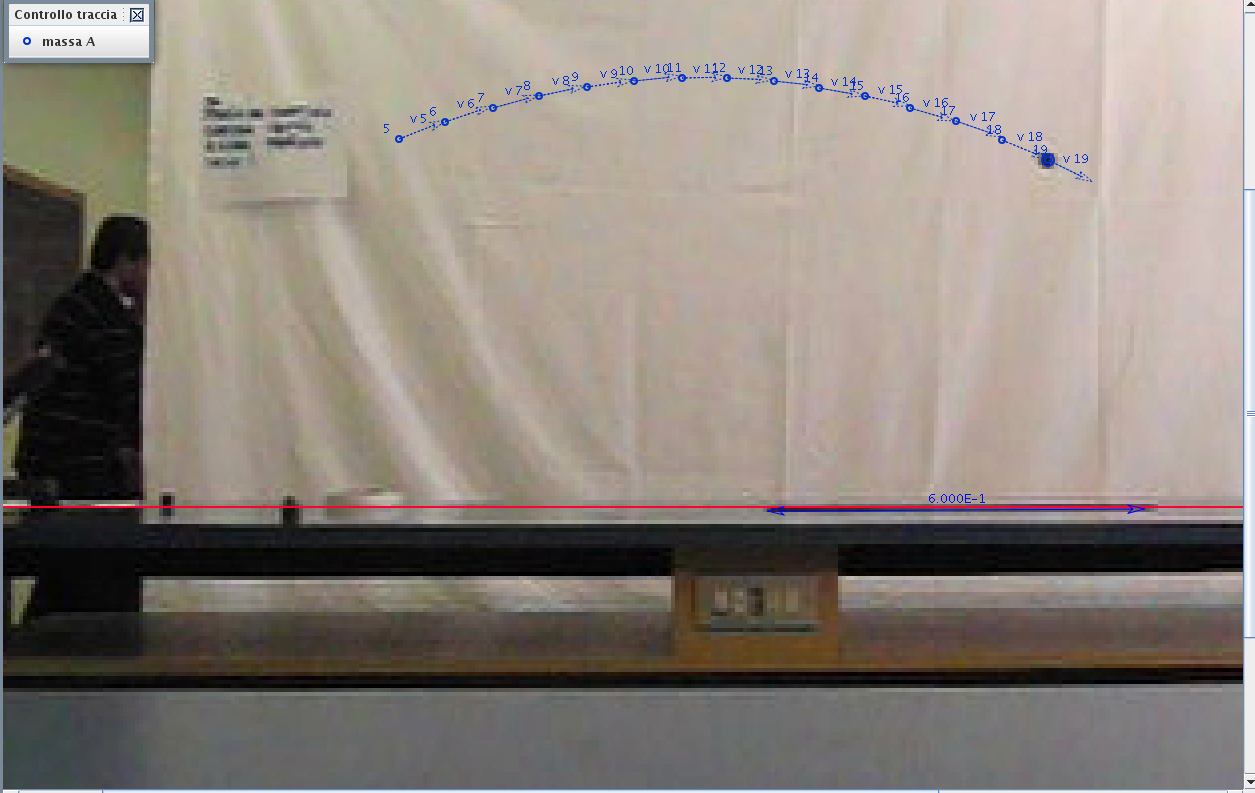
\includegraphics[width=0.8\textwidth]{./immagini/tracker_visualizzazione_velocita.png}
 % tracker_visualizzazione_velocita.png: 1255x793 pixel, 72dpi, 44.27x27.97 cm, bb=0 0 1255 793
 \caption{Rappresentazione dei vettori velocità media della particella durante il volo}
 \label{fig:visualizzazione_vel}
\end{figure}

\begin{figure}[H]
 \centering
 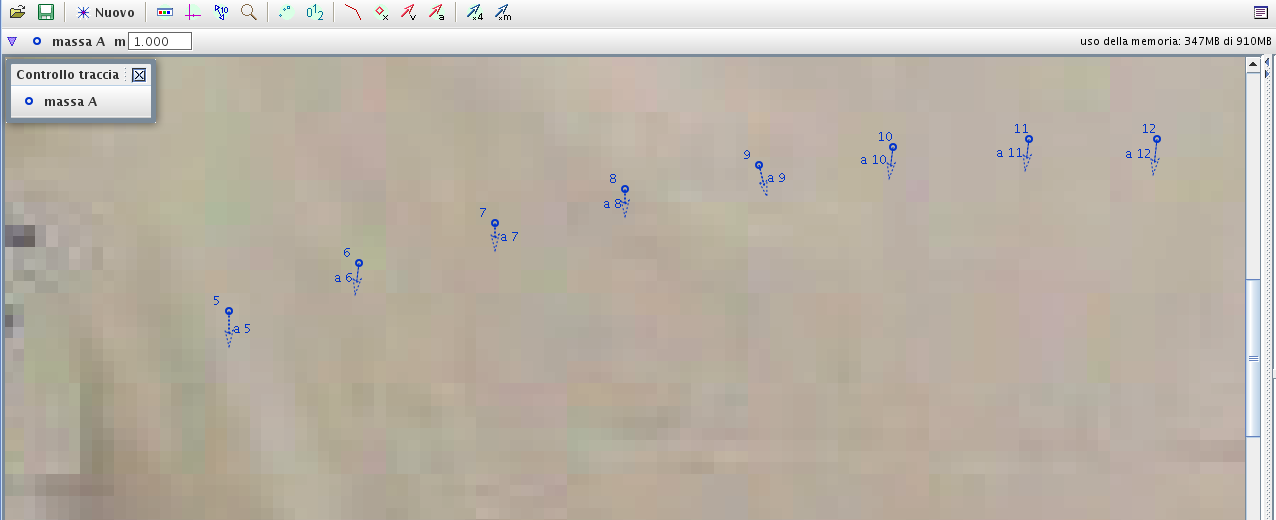
\includegraphics[width=0.8\textwidth]{./immagini/tracker_visualizzazione_accelerazione.png}
 % tracker_visualizzazione_accelerazione.png: 1276x520 pixel, 72dpi, 45.01x18.34 cm, bb=0 0 1276 520
 \caption{Reppresentazione dei vettori accelerazione media della particella}
 \label{fig:vettori_acc}
\end{figure}

\subsection*{Traccia \emph{Vettore}}

In molti casi può essere utile sovrapporre dei vettori al  filmato, nell'esempio del cannone possiamo utilizzare lo strumento \emph{Vettore} per misurare l'inclinazione del cannone e dedurre quindi la direzione della velocità iniziale. In Tracker i vettori non sono altro che un nuovo tipo di traccia, agiremo quindi come abbiamo fatto per il \emph{Punto Massa}, clicchiamo su \emph{Nuovo} nella barra delle icone e scegliamo \emph{Vettore}, fatto ciò tenendo premuto il tasto \textsl{shift} trasciniamo il vettore con il mouse fino a farlo coincidere con il corpo del cannone. Nella tabella di destra potrete leggere i valori delle componenti del vettore e la sua inclinazione in radianti.

\begin{figure}[H]
 \centering
 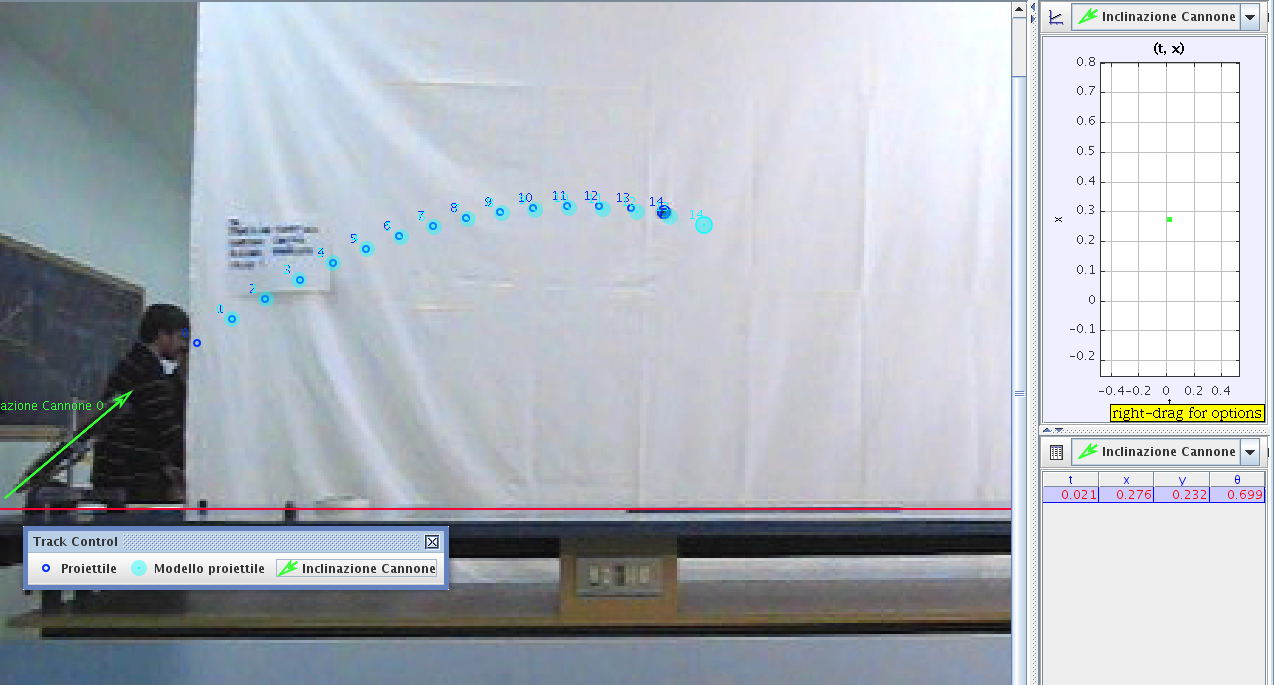
\includegraphics[width=0.8\textwidth]{./immagini/inclinazione_cannone.png}
 % inclinazione_cannone.png: 1274x685 pixel, 72dpi, 44.94x24.16 cm, bb=0 0 1274 685
 \caption{Tramite lo strumento \emph{Vettore} possiamo misurare l'inclinazione del cannone al momento del lancio}
 \label{fig:inclinazione_cannone}
\end{figure}


\subsection*{Esportazione dei dati}

L'esportazione dei dati da Tracker è molto semplice, selezioniamo la traccia di cui vogliamo esportare le misure, selezioniamo le misure da esportare con il mouse nella tabella di destra, figura [\ref{fig:export_dati}] e quindi tramite il menu accessibile cliccando il tasto destro del mouse sull'area selezionata, eseguiamo il comando \emph{Copia dati}. Le nostra misure si trovano ora nella memoria del computer, tramite il comando incolla di qualsiasi altra applicazione possiamo riutilizzare i dati estratti tramite Tracker.

\begin{figure}[H]
 \centering
 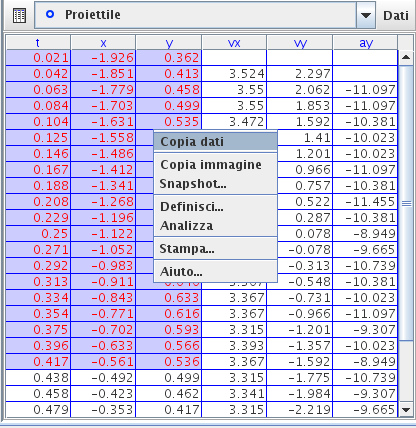
\includegraphics[width=0.8\textwidth]{./immagini/export_dati_ita.png}
 % export_dati_ita.png: 416x428 pixel, 75dpi, 14.09x14.49 cm, bb=0 0 399 411
 \caption{Per esportare i dati clicchiamo con il tasto destro su una sezione evidenziata e selezioniamo la voce \emph{Copia dati}}
 \label{fig:export_dati}
\end{figure}







\subsection*{Analisi dei dati}

I dati relativi alle posizioni del proiettile nei vari frame del filmato sono ora disponibili per essere ulteriormente analizzati. Per visualizzare i dati raccolti clicchiamo sul menu \textsl{Finestra} e mettiamo una spunta su \textsl{Vista destra}. Nella parte destra della finestra principale di Tracker troveremo ora una tabella contenente i dati raccolti e un grafico cartesiano. Cliccando sulle etichette degli assi del grafico potremo variare le quantità graficate, in figura [\ref{fig:grafico_traiettoria}] è riportata la traiettoria ovvero il grafico $y(x)$. Nel grafico di figura [\ref{fig:tracker_accelerazione}] possiamo invece vedere l'andamento dalla componente $y$ dell'accelerazione media del proiettile in funzione del tempo $t$ la figura [\ref{fig:tracker_velocita_verticale}] ci mostra come varia nel tempo la componente verticale della velocità media del proiettile, notiamo che l'andamento del grafico può essere ben approssimato da una linea retta in ottimo accordo con la previsione teorica di moto uniformemente accelerato.

\begin{figure}[H]
 \centering
 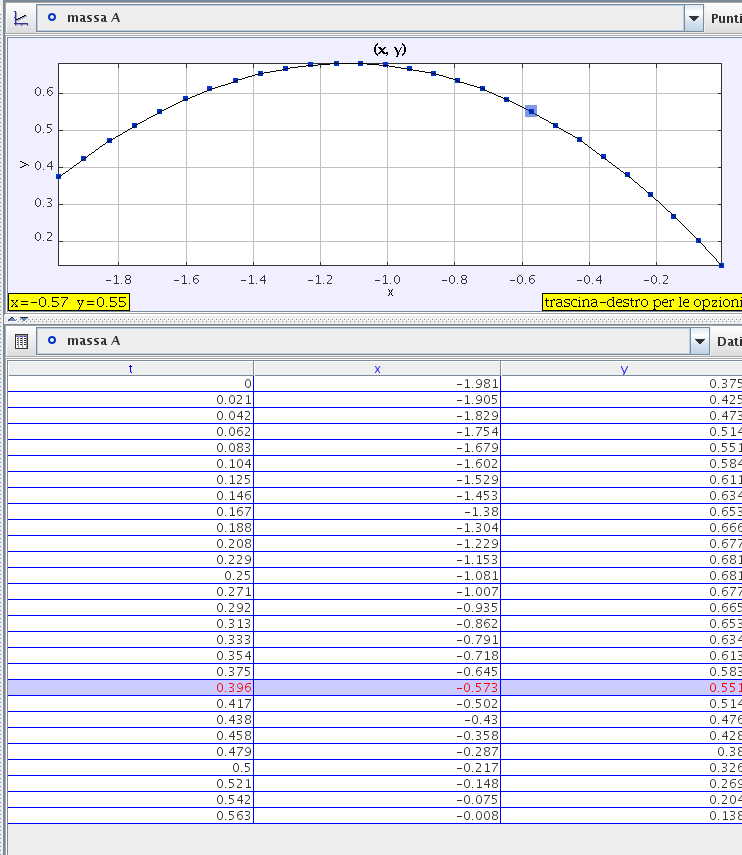
\includegraphics[width=0.5\textheight]{./immagini/tracker_grafico_traiettoria.png}
 % tracker_grafico_traiettoria.png: 742x855 pixel, 72dpi, 26.17x30.16 cm, bb=0 0 742 855
 \caption{Cliccando su Finestra \RIGHTarrow Vista destra possiamo rappresentare i dati raccolti durante la procedura di tracciamento del proiettile}
 \label{fig:grafico_traiettoria}
\end{figure}


\begin{figure}[H]
 \centering
 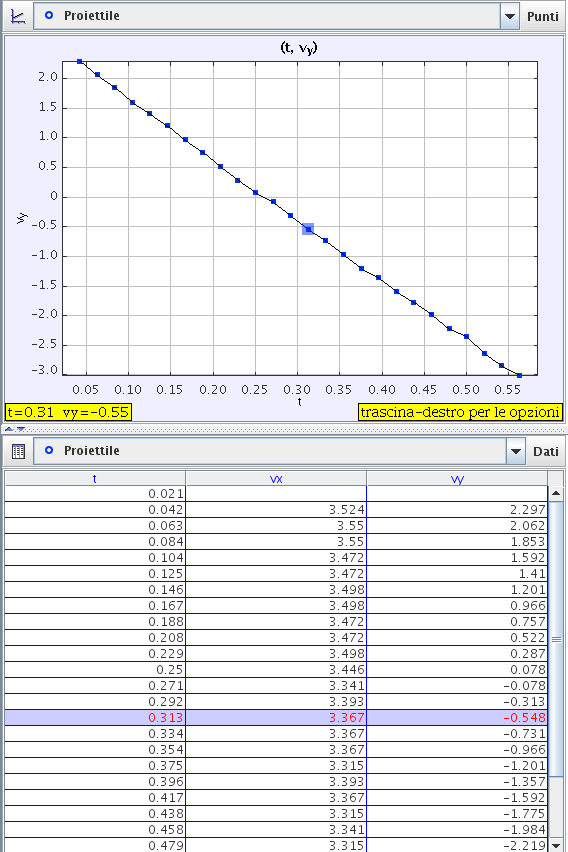
\includegraphics[width=0.8\textwidth]{./immagini/velocita2.png}
 % tracker_velocità verticale.png: 760x863 pixel, 72dpi, 26.81x30.44 cm, bb=0 0 760 863
 \caption{Valori per la velocità nella direzione y calcolati da Tracker}
 \label{fig:tracker_velocita_verticale}
\end{figure}


\begin{figure}[H]
 \centering
 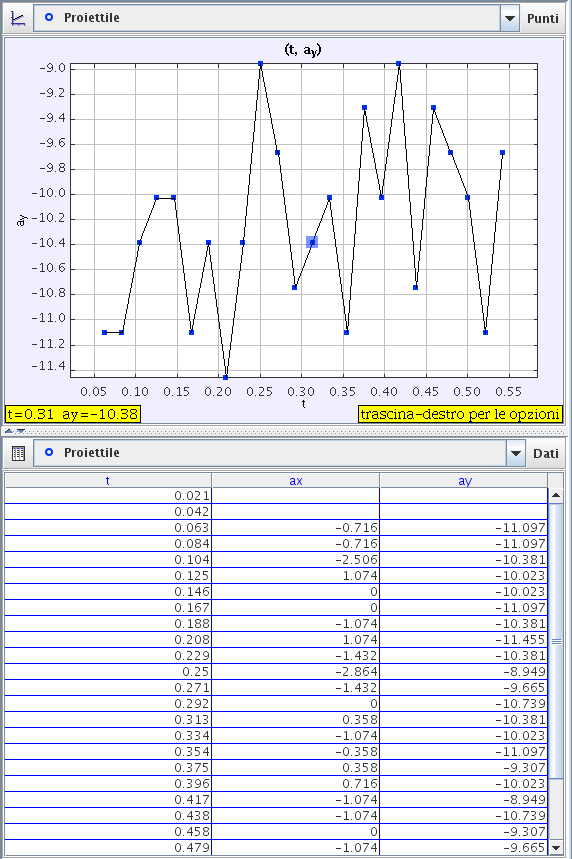
\includegraphics[width=0.8\textwidth]{./immagini/accelerazione2.png}
 % tracker_accelarazione.png: 752x858 pixel, 72dpi, 26.53x30.26 cm, bb=0 0 752 858
 \caption{Valori calcolati per l'accelerazione media del proiettile}
 \label{fig:tracker_accelerazione}
\end{figure}

Una domanda sorge ora lecita, il moto del proiettile è effettivamente un moto parabolico? Di quanto la traiettoria filmata si discosta dalla previsione teorica? Per rispondere a questi interessanti quesiti Tracker ci mette a disposizione due modelli analitici con i quali possiamo simulare il comportamento di un proiettile ideale. Per provare a sovrapporre la previsione teorica alla nostra ripresa creiamo una nuova traccia cliccando sul pulsante \textsc{Nuovo} nella barra delle icone e scegliendo \RIGHTarrow Modello di particella dinamico \RIGHTarrow Cartesiano. Nella finestra controllo traccia comparirà un nuovo elemento rappresentativo della simulazione figura [\ref{fig:particella_dinamica}]


\begin{figure}[H]
 \centering
 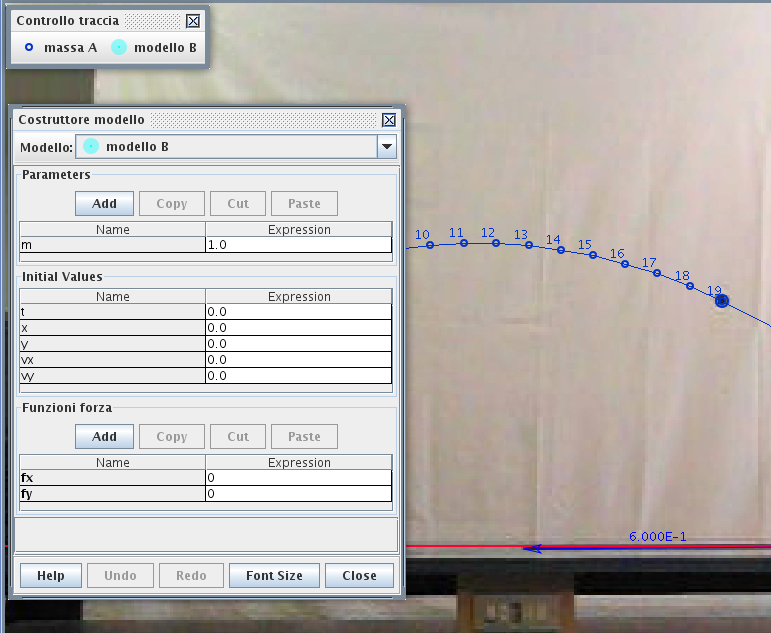
\includegraphics[width=\textwidth]{./immagini/tracker_nuovo_modello_particella_dinamico.png}
 % tracker_nuovo_modello_particella_dinamico.png: 1280x962 pixel, 72dpi, 45.15x33.93 cm, bb=0 0 1280 962
 \caption{Creaiamo un modello matematico per la descrizione del nostro sistema, dalla barra delle icone Nuovo \RIGHTarrow Modello di particella dinamico \RIGHTarrow Cartesiano}
 \label{fig:particella_dinamica}
\end{figure}

Nella finestra di dialogo dovremo inserire i valori che modellano il nostro esperimento, nella sezione parametri inseriremo la massa $m$\footnote{L'esempio in esame è invariante rispetto alla massa} e il valore dell'accelerazione di gravità $g$, nella sezione parametri iniziali inseriremo la posizione e la velocità\footnote{Nota, per i valori della velocità al tempo zero possiamo utilizzare una differenza in avanti} al tempo iniziale,  nel caso in esame sarà $t_0=0s$. I valori iniziali dovranno essere letti nella tabella relativa alla traccia reale
Come ultima cosa inseriamo le componenti della forza $f_x=0$ e $f_y=-mg$ figura [\ref{fig:model_builder}]. 


\begin{figure}[H]
 \centering
 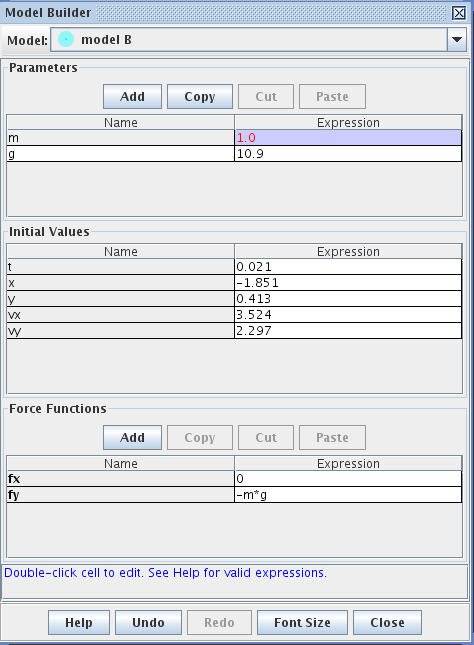
\includegraphics[width=0.6\textwidth]{./immagini/tracker_model_builder.png}
 % tracker_model_builder.png: 474x645 pixel, 72dpi, 16.72x22.75 cm, bb=0 0 474 645
 \caption{Interfaccia per la creazione del modello del moto del proiettile}
 \label{fig:model_builder}
\end{figure}

Non appena tutti i dati necessari all'integratore, per risolvere la seconda equazione di Newton saranno stati inseriti verranno disegnate sullo schermo le posizioni teoriche del proiettile in un determinato istante di tempo


\begin{figure}[H]
 \centering
 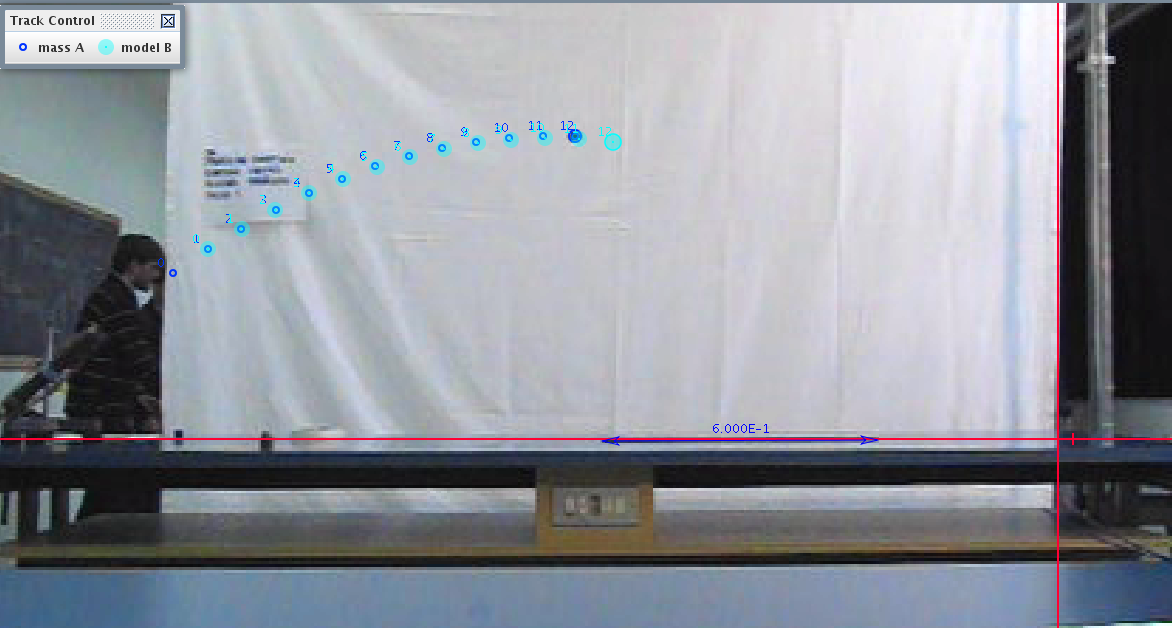
\includegraphics[width=\textwidth]{./immagini/tracker_model_over_data.png}
 % tracker_model_over_data.png: 1278x962 pixel, 72dpi, 45.08x33.93 cm, bb=0 0 1278 962
 \caption{Sovrapposizione del modello calcolato risolvendo la seconda equazione di Newton ai dati sperimentali}
 \label{fig:model_over_data}
\end{figure}


\begin{figure}[H]
 \centering
 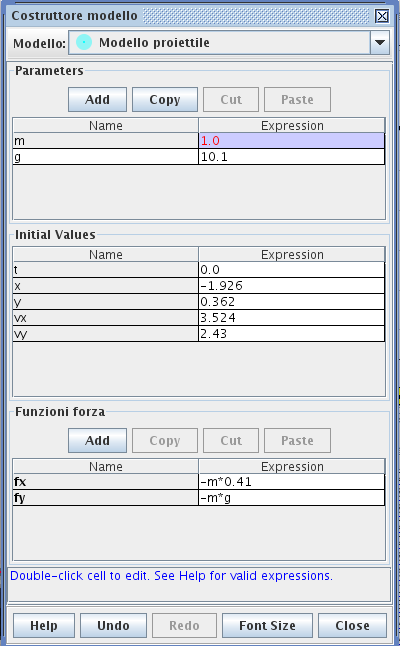
\includegraphics[width=0.6\textwidth]{./immagini/tracker_model_builder2.png}
 % tracker_model_builder2.png: 400x646 pixel, 72dpi, 14.11x22.79 cm, bb=0 0 400 646
 \caption{Introducendo un forza in grado di diminuire la velocità orizzontale del proiettile siamo in grado di modellare il frenamento dell'aria sulla pallina}
 \label{fig:model_builder2}
\end{figure}



\begin{thebibliography}{9}
\bibitem{NumericalRecipies} Numerical Recipies \emph{The art of scientific Computing  3rd Edition}
\bibitem{Laboratorio7} Laboratorio Cinematica II \url{http://cartan.e-moka.net/Fisica/Laboratorio/Laboratorio-7-cinematica-bidimensionale}
\end{thebibliography}



\end{document}
